
%(BEGIN_QUESTION)
% Copyright 2014, Tony R. Kuphaldt, released under the Creative Commons Attribution License (v 1.0)
% This means you may do almost anything with this work of mine, so long as you give me proper credit

Identify which of these components are connected directly in series with each other, and which are connected directly in parallel with each other:

$$\includegraphics[width=15.5cm]{i01164x01.eps}$$

Assume that the open wire ends are connection points to a power source.  In circuits where ground symbols appear, consider ground as the other side of the power source.  

\underbar{file i01164}
%(END_QUESTION)





%(BEGIN_ANSWER)

\noindent
{\bf Figure 1:}

R1 in series with SW1.

\vskip 10pt

\noindent
{\bf Figure 2:}

R1 in series with R2; R3 in parallel with R4.

\vskip 10pt

\noindent
{\bf Figure 3:}

R1 parallel with R2.

\vskip 10pt

\noindent
{\bf Figure 4:}

R1 parallel with R2.

\vskip 10pt

\noindent
{\bf Figure 5:}

L1 in series with C1.

\vskip 10pt

\noindent
{\bf Figure 6:}

R3 in parallel with R4.

%(END_ANSWER)





%(BEGIN_NOTES)

Work with your students to clearly identify rules by which series and parallel connections may be identified.  This is extremely important for students to grasp if they are to be successful analyzing series-parallel networks of any kind.  The most common problems I encounter as an electronics instructor with reference to series-parallel are invariably related to students' lack of ability to consistently distinguish series sub-networks and parallel sub-networks in series-parallel combination circuits.

%INDEX% Electronics review: series-parallel circuits

%(END_NOTES)


